\section{Cloning} \label{sec:cloning}
\subsection{Overview}
The master image for lab loads is very important, but just as important is the method for deployment.  With the number of machines we have present in the labs, installing each machine individually would require far more time than we have available.  In addition, because of human error, many inconsistencies between lab machines would appear.  Instead, we define a method to copy the master image to the rest of the labs.  We do this by copying the lab image to a file and moving that file to a server that the lab workstations can access.  The specific instructions we follow to do this can be found in Appendix~\ref{ap:lab_installation}.

\subsection{Setup and Preparation}
In our labs, the master image file is moved to the Print Servers.  The Print Servers have to be set up with DHCP, TFTP, PXE, and NFS.  Specific instructions for this process can be found in the Print Server section.  The image must be copied to the NFS export directory on each Print Server in each lab.  We have tried using a central server that all workstations access for the image, however, this caused all workstations to compete for the bandwidth given by one switch.  This slowed the process down significantly.  By deploying the image to each Print Server, it allows the bandwidth used to be isolated within each lab subnet.  All labs can then be imaged in parallel.  

Deployment of the image requires configuring the workstations to boot from network.  The clients must have their BIOS setup so that netbooting is enabled and is first priority.  It may also be a good idea to disable other booting options since they are unnecessary for clones and could pose a security risk.  The BIOS should also be passworded to prevent changes.  Technically, the BIOS password can be reset by opening the machine and setting a jumper, but in our environment, the workstation cases are locked so that the jumper is inaccessible.  

\subsection{Deploying the Clone Image}
The workstations can be booted one by one to load a temporary network image.  It will load a bootloader first to determine what operating system to finish booting with.  The top option will likely just be to boot from the local hard disk.  Another option we show is to boot from network (and there may be multiple network images).  The image to clone with is just a variation of the distribution installer modified to be used for cloning.  It contains the clone script and any other tools for use in cloning.  Before the clone script can be run, the hard disk will need to be partitioned manually once.  This is per hard disk not per clone operation, so once it is finished, it does not need to be done again until hardware changes.  Once the formatting is done, the script can be run while booted from network.

This script does several things to prepare, deploy, and configure the clone image.  It takes a single argument of the last octet of the workstation's IP address.  It first enables networking if it is not already enabled.  Then it sets the machines address temporarily to the one it was given in an argument.  It then sets the default gateway for the lab.  This could require either a second argument to the script or separate scripts for each lab subnet (we use the latter for convenience).  It then runs filesystem tools to make a new file system and a swap area to the partitions.  It then mounts the hard drive partitions to a local mount point.  It will also need to mount the NFS export directory of the Print Server so that it can access the master image.  The master image is in compressed tarball format.  Once it can reach this file via a network mount, it can untar the image onto the local hard disk.  This is the longest step.  After it is finished, two more mount commands are needed to bind the process and system directories of the new image.  After that, the bootloader, LILO, runs to install the bootloader into the boot sector of the hard drive. 

At this point, the system is bootable.  It is not yet configured to be unique though.  The last thing the script does is set the hostname and the permanent IP address by editing the configuration files on the hard disk partitions.  On some systems, the monitor may not work with the defaults the master image had.  If so, the appropriate configuration files are changed to update that.  Some other configurations may need to be changed, but these vary for each distribution and release so we have no way of documenting them.  The script edits the ``/etc/printcap" file and sets the default printer to be the one in the room in which the workstation is located.  All workstations in a room are clones except for the printserver.  Figure~\ref{fig:RoomNetworkLayout} shows our lab layout. 

\begin{figure}
  \begin{center}
    \scalebox{0.7}{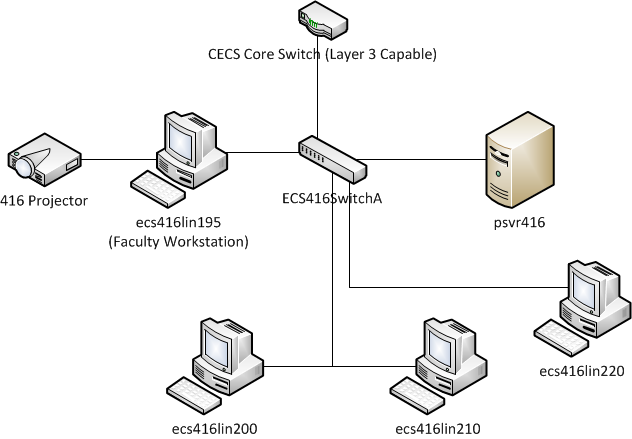
\includegraphics{../figures/RoomNetworkLayout.png}}
  \end{center}
  \caption{Lab layout.}
  \label{fig:RoomNetworkLayout}
\end{figure}

\
\vskip1pt
\ 

\subsection{Cloning Efficiency and Potential Improvements}
This system is fairly efficient and only requires about 2 hours to clone all three of our labs if cloned in parallel.  The only interaction between the sysadmin and each clone is to run the clone script with the IP address of the machines.  This process could be improved though.  To do so, every workstation needs to have its MAC address copied to the Print Server's DHCP table.  In addition, a copy of this table would need to be available during the netboot since the small netboot image does not usually have a DHCP client.  This would then prevent the need for the sysadmin to enter the address since every machine would be uniquely identified by MAC address.  This can be further automated by broadcasting wakeonlan packets from the Print Servers to the machines to start them.  This would prevent the need for the sysadmin to even enter the lab at all.  

All of these improvements only work to the benefit of the system administrator though.  They do not lessen the time it takes for the labs to deploy from two hours.  To this, the biggest bottleneck, network bandwidth, would have to be addressed.  The expensive solutions is to do switch upgrades.  Currently, we use 100MB managed HP switches.  We could update them to 1GB (1000MB) switches and that may cut the time down significantly.  However, there are two inexpensive solutions.  The first is to enable QOS (Quality of Service) on our managed switches.  This would force the bandwidth to be evenly distributed across machines whereas currently one machine can take most of the bandwidth and slow all other machines down.  QOS requires managed switches to support it.   The scripts could further be timed such that the machines stagger their installs.  We could send wakeonlan packets to each workstation on a timer, allowing each machine five minutes to get high bandwidth before others start competing for it.  As more machines enter, machines that started earlier finish.  Five minutes may not be the ideal time.  That can be optimized with each successive cloning session.  These improvements may or may not work as expected because we have not tested them yet.  Fatal drawbacks may be discovered during testing.  

